%%%%%%%%%%%%%%%%%%%%%%%%%%%%%%%%%%%%%%%%%%%%%%%%%%%%%%%%%%%%%%%%%%%%%%
% How to use writeLaTeX: 
%
% You edit the source code here on the left, and the preview on the
% right shows you the result within a few seconds.
%
% Bookmark this page and share the URL with your co-authors. They can
% edit at the same time!
%
% You can upload figures, bibliographies, custom classes and
% styles using the files menu.
%
%%%%%%%%%%%%%%%%%%%%%%%%%%%%%%%%%%%%%%%%%%%%%%%%%%%%%%%%%%%%%%%%%%%%%%

\documentclass[12pt]{article}

\usepackage{sbc-template}
\usepackage{graphicx,url}
\usepackage{float}
\usepackage{array}
\usepackage{tabularx}
\usepackage{makecell}

\usepackage{tcolorbox}
\usepackage{minted}

\usepackage[utf8]{inputenc}  

\tcbset{
  codeSnippetStyle/.style={
    colback=gray!10, % cor de fundo mais clara
    colframe=gray!30!, % cor da borda
    title=#1, % título da caixa
    coltitle=black, % cor do título
    boxrule=0.2mm, % espessura da borda
    arc=3mm, % arredondamento dos cantos
    width=\textwidth, % largura da caixa
    boxsep=7pt
  }
}

\newcolumntype{Y}{>{\centering\arraybackslash}X}

\sloppy

%\title{INVESTIGAÇÃO DA ADESÃO DE BOAS PRÁTICAS DE DESENVOLVIMENTO EM PROJETOS OPEN SOURCE FLUTTER: UMA ANÁLISE DE CÓDIGO E MANUTENIBILIDADE}

\title{Análise da Aderência às Boas Práticas de Desenvolvimento em Projetos Open Source Flutter: Primeiros Insights}
\author{Anonymous\inst{1}}

\address{Anonymous \email{\{anonymous\}@anonymous}}

\begin{document} 

\maketitle

\begin{abstract}
This research investigates adherence to best development practices in open-source Flutter projects, focusing on code quality and maintainability. We analyzed 45 projects using SonarQube to identify Best Practice Violations (BPVs). A total of 10,120 BPVs were found, distributed across three severities: 5,149 Minor, 4,273 Major, and 698 Critical. We calculated the Pearson correlation coefficient to confirm the relationship between BPVs and non-commenting lines of code (NCLOC) and between BPVs and cyclomatic complexity. We observed a strong correlation (0.8978) between BPVs and NCLOC, and a moderate correlation (0.4509) between BPVs and complexity. These findings highlight areas for Flutter developers to improve code quality.
\end{abstract}
     
\begin{resumo} 
Esta pesquisa investiga a adesão às melhores práticas de desenvolvimento em projetos open-source Flutter, focando na qualidade e manutenibilidade do código. Analisamos 45 projetos utilizando SonarQube para identificar Violações de Boas Práticas (VBPs). Foram encontradas 10.120 VBPs, distribuídas em três severidades: 5.149 Leves, 4.273 Graves e 698 Críticas. Calculamos o coeficiente de correlação de Pearson para confirmar a relação entre VBPs e linhas de código (LCNC) e entre VBPs e complexidade ciclomática. Observamos uma correlação forte (0.8978) entre VBPs e LCNC, e uma correlação moderada (0.4509) entre VBPs e complexidade. Esses achados destacam áreas para os desenvolvedores Flutter melhorarem a qualidade do código.
\end{resumo}

\section{Introdução}
A evolução tecnológica acelerada tem modificado substancialmente nossa interação com o mundo digital, com os dispositivos móveis emergindo como agentes principais dessa transformação. No Brasil, a média de 1,2 smartphones por habitante causa uma demanda crescente por serviços digitais e aplicativos móveis. Em 2022, por exemplo, os investimentos em tecnologia da informação (TI) corresponderam a 9\% do faturamento das empresas, refletindo também em um aumento significativo no desenvolvimento de aplicativos móveis \cite{FGVcia2023}.

Lançado pelo Google em 2017, o Flutter é um \textit{framework} de código aberto que se tornou popular por permitir que desenvolvedores criem aplicativos que funcionam em múltiplos sistemas operacionais, como Android e iOS, com mínimas alterações no código-fonte, tornando-se uma escolha popular para desenvolvimento multiplataforma \cite{flutter}. Utilizando a linguagem de programação Dart, também desenvolvida pelo Google, o Flutter facilita a escrita de código de alta qualidade e a manutenção a longo prazo. Além disso, se destaca pelo motor gráfico próprio, que oferece consistência e desempenho em diferentes plataformas, e pelo rico ecossistema de pacotes e plugins disponível no Pub, o gerenciador de pacotes do Dart.

Para garantir que os aplicativos desenvolvidos com Flutter mantenham sua robustez e sejam facilmente mantidos ao longo do tempo, é essencial adotar as melhores práticas de desenvolvimento. No contexto do Flutter, isso inclui seguir recomendações da equipe principal do Dart, como a legibilidade, consistência, concisão e eficiência do código \cite{dartBestPractices}. Princípios de código limpo, como clareza, simplicidade e eficiência, além de técnicas de refatoração contínua \cite{fowler1999refactoring}, são fundamentais para assegurar a qualidade técnica do software e facilitar sua manutenção contínua.

Este estudo investiga a adesão às melhores práticas de programação recomendadas pelo time principal do Dart em projetos open source desenvolvidos com Flutter. Este estudo visa responder as seguintes questões de pesquisa:
\begin{enumerate}
\item Qual a prevalência de violações das melhores práticas recomendadas?
\item Com que frequência essas práticas são violadas?
\item Quais tipos de práticas são mais frequentemente violadas?
\end{enumerate}

\section{Metodologia}

Esta seção detalha o procedimento utilizado para avaliar a incidência e o impacto de violações de boas práticas (VBPs) em projetos open source desenvolvidos com Flutter. A metodologia é estruturada em quatro etapas principais: seleção de projetos, configuração das ferramentas de análise, coleta de dados e avaliação dos resultados. Além das VBPs, também analisamos a complexidade do código dos projetos, medida por métricas como a complexidade ciclomática e número de linhas de código não comentadas (LCNC) \cite{mccabe1976complexity}, para avaliar a qualidade dos projetos Flutter.

\subsection{Seleção de Projetos}
A seleção apropriada dos projetos é crucial para garantir a relevância da pesquisa.Inicialmente, foram considerados 152 projetos open source Flutter recomendados pela comunidade e disponíveis no repositório \textit{Open-Source Flutter Apps}\footnote{Tortuvshin Bayarsaikhan. Open-Source Flutter Apps. 2023. Disponível em: \url{https://github.com/tortuvshin/open-source-flutter-apps}. Acessado em: 08 de julho de 2024}. Aplicamos critérios específicos para filtrar esses projetos, resultando em uma amostra final de 50 projetos relevantes para análise:
\begin{enumerate}
    \item No mínimo 30 commits, garantindo múltiplas atualizações.
    \item Último commit feito nos últimos 3 anos, assegurando atividade recente.
    \item Mínimo de 30 estrelas no GitHub, indicando relevância na comunidade.
\end{enumerate}

\subsection{Configuração das Ferramentas de Análise}
Utilizamos o SonarQube, uma plataforma reconhecida por sua capacidade de análise de código, para identificar VBPs. O SonarQube foi instalado em um container Docker para garantir um ambiente de análise controlado e consistente. Também configuramos o SonarScanner para coletar dados detalhados dos projetos.

\subsection{Execução da Análise}
A análise foi realizada utilizando o SonarScanner, configurado com um arquivo \texttt{sonar-project.properties} específico para cada projeto. Foram coletadas métricas como número de VBPs, severidade e complexidade ciclomática. A tabela abaixo resume os passos principais:
\begin{enumerate}
    \item Configuração do ambiente Docker e instalação do SonarQube.
    \item Baixando e instalando o plugin para análise de Dart e Flutter.
    \item Configuração e execução do SonarScanner nos projetos selecionados.
\end{enumerate}

\subsection{Coleta e Armazenamento de Dados}
Os dados foram coletados através da API do SonarQube e armazenados em formato JSON. Utilizamos scripts em Python para automatizar a coleta, tratamento e análise dos dados, garantindo consistência e precisão nos resultados.

\subsection{Análise dos Resultados}
Os resultados foram analisados para identificar a prevalência e severidade das VBPs. Calculamos o coeficiente de correlação de Pearson para avaliar a relação entre VBPs e Linhas de Código Não Comentadas (LCNC) e entre VBPs e complexidade ciclomática. Os dados foram visualizados por gráficos e tabelas para facilitar a interpretação.

\section{Resultados}

Esta seção apresenta os resultados obtidos a partir da análise dos projetos open source desenvolvidos com Flutter, com foco na avaliação da adesão às melhores práticas de desenvolvimento. Foram analisados 45 projetos utilizando o SonarQube para identificar VBPs. No total, foram encontradas 10.120 VBPs, distribuídas em três níveis de severidade: 5.149 violações menores, 4.273 violações maiores e 698 violações críticas.

\subsection{Correlação entre VBPs, Linhas de Código Não Comentadas (LCNC) e Complexidade Ciclomática}
Calculamos o coeficiente de correlação de Pearson para avaliar a relação entre VBPs e o número de LCNC, bem como entre VBPs e complexidade ciclomática. Observamos uma correlação forte (\textit{r} = 0.8978) entre VBPs e LCNC, indicando que mais linhas de código estão associadas a mais VBPs. Adicionalmente, uma correlação moderada (\textit{r} = 0.4509) foi encontrada entre VBPs e complexidade ciclomática, sugerindo que projetos com maior complexidade ciclomática tendem a ter mais VBPs.

\begin{figure}[H]
\centering
\includegraphics[width=0.45\textwidth]{vbps_vs_lcnc.png}
\includegraphics[width=0.45\textwidth]{vbps_vs_complexidade.png}
\caption{Correlação entre VBPs e LCNC (esquerda) e entre VBPs e Complexidade Ciclomática (direita)}
\label{fig
}
\end{figure}

\subsection{Regras Mais Violadas}
Esta subseção apresenta as cinco regras de boas práticas mais frequentemente violadas nos projetos analisados. A Figura~\ref{fig
} mostra a distribuição dessas regras, facilitando a visualização das principais áreas problemáticas nos projetos Flutter.

\begin{figure}[H]
\centering
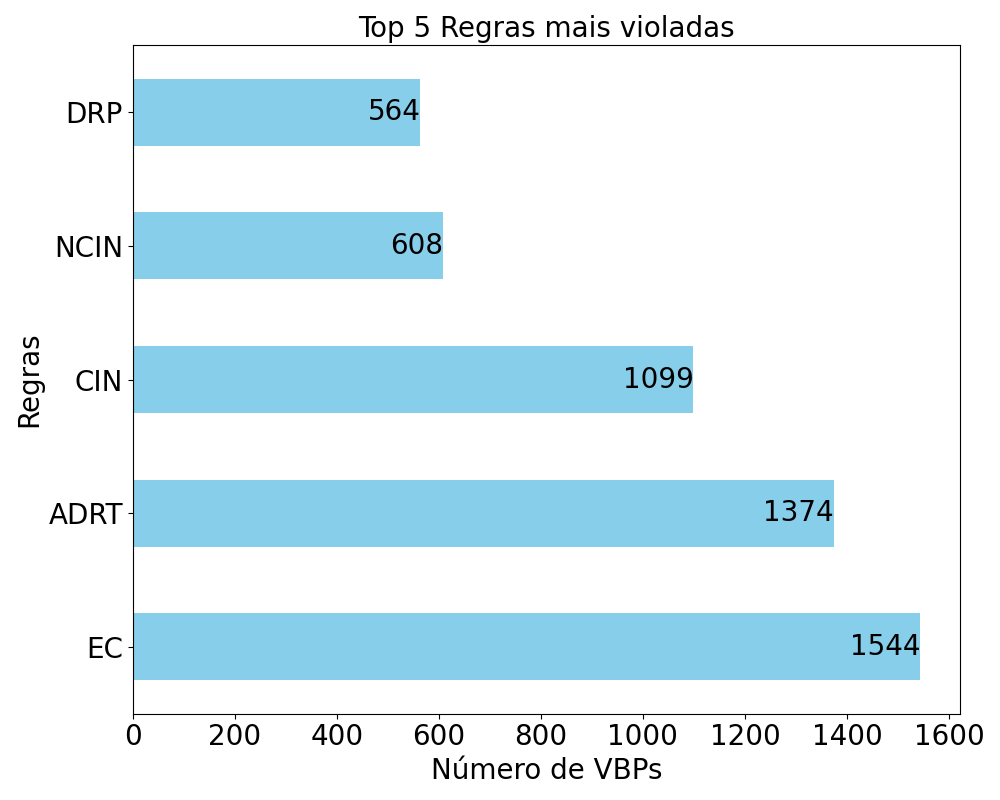
\includegraphics[width=.5\textwidth]{rule_distribution.png}
\caption{Distribuição das Regras Mais Violadas}
\label{fig:rule_distribution}
\end{figure}

As siglas usadas no gráfico representam: \textbf{EC}: \textit{Exhaustive Cases}, verifica se todas as possibilidades em uma enumeração são cobertas; \textbf{ADRT}: \textit{Always Declare Return Types}, garante que todas as funções tenham tipos de retorno declarados; \textbf{CIN}: \textit{Constant Identifier Names}, verifica se os nomes das constantes estão em conformidade com as convenções de nomenclatura; \textbf{NCIN}: \textit{Non Constant Identifier Names}, verifica se os nomes dos identificadores não constantes estão em conformidade com as convenções de nomenclatura; \textbf{DRP}: \textit{Depend on Referenced Packages}, garante que as dependências declaradas estejam sendo utilizadas.

% Esses dados indicam haver uma necessidade significativa de melhorar a adesão a práticas fundamentais de codificação, como garantir que todas as possibilidades em enumerações sejam cobertas, declarar explicitamente os tipos de retorno de funções, e seguir as convenções de nomenclatura tanto para constantes quanto para identificadores não constantes.

\subsection{Exemplo de Violação Crítica: Always Declare Return Types (ADRT)}
Entre as regras mais frequentemente violadas, a prática de declarar explicitamente os tipos de retorno de métodos (\textbf{ADRT}) se destaca por sua importância na manutenção e compreensão do código.

No exemplo abaixo, o método \texttt{getUserType} não possui um tipo de retorno declarado, o que pode levar a problemas de manutenção e compreensão do código:

\begin{tcolorbox}[codeSnippetStyle={gsy\_github\_app\_flutter/lib/page/my\_page.dart}]
\begin{minted}[breaklines, fontsize=\footnotesize]{dart}
getUserType() {
  if (_getStore()?.state.userInfo == null) {
    return null;
  }
  return _getStore()?.state.userInfo?.type;
}
\end{minted}
\end{tcolorbox}

Ao invés disso, o método deveria declarar explicitamente o tipo de retorno, como mostrado abaixo:

\begin{tcolorbox}[codeSnippetStyle={}]
\begin{minted}[breaklines, fontsize=\footnotesize]{dart}
String? getUserType() {
  if (_getStore()?.state.userInfo == null) {
    return null;
  }
  return _getStore()?.state.userInfo?.type;
}
\end{minted}
\end{tcolorbox}

\section{Discussão}
Os resultados desta pesquisa mostram uma forte correlação entre o número de VBPs e as linhas de código não comentadas (LCNC), indicando que projetos maiores tendem a apresentar mais violações. Também foi observada uma correlação moderada entre VBPs e complexidade ciclomática, sugerindo que a complexidade do código influencia a qualidade do software.

Esses achados são consistentes com a literatura, que destaca a importância de práticas de codificação estruturada para a manutenibilidade do software \cite{hunt1999pragmatic}. As regras mais violadas, como Exhaustive Cases e Always Declare Return Types, indicam áreas onde os desenvolvedores devem concentrar esforços para melhorar a qualidade do código.

Recomendamos o uso de ferramentas de lint e análise de código, como SonarQube e Dart Analyzer, durante o desenvolvimento. Essas ferramentas podem identificar violações de boas práticas em tempo real, permitindo correções antes que se tornem significativas. A integração dessas ferramentas no processo de desenvolvimento contínuo pode ajudar a manter a qualidade do código, reduzir a complexidade ciclomática e evitar a duplicação de código \cite{martin2011clean}.

\section{Conclusão}
Esta pesquisa analisou 45 projetos open-source Flutter para identificar Violações de Boas Práticas (VBPs), encontrando mais de 10.000 violações distribuídas entre diferentes severidades.

Principais achados:
\begin{itemize}
\item Forte correlação entre VBPs e LCNC, indicando mais violações em projetos maiores.
\item Correlação moderada entre VBPs e complexidade ciclomática, sugerindo a importância de controlar a complexidade do código.
\item Identificação das regras mais violadas, fornecendo áreas focais para melhorias na qualidade do código.
\end{itemize}

Esses resultados destacam áreas específicas onde melhorias podem ser feitas para aderir melhor às práticas recomendadas e melhorar a qualidade e manutenibilidade do código em projetos Flutter.

Para futuros trabalhos, recomendamos uma análise mais detalhada das causas das violações de boas práticas e a investigação de técnicas automatizadas para auxiliar os desenvolvedores a aderirem a essas práticas. Expandir o conjunto de dados para incluir mais projetos e explorar a eficácia de diferentes ferramentas e metodologias de análise de código também seria benéfico.



\bibliographystyle{sbc}
\bibliography{sbc-template}

\end{document}
